\section{Baselines and Methods}
\label{sec:exp}

%% 1. 简要再次介绍数据集

All experiments are performed using UAV-BD, the training, validation and testing date include $ 16258 $, $ 4065 $ and $ 5081 $ images, respectively. Note that the images for training, testing and validation are the size of $ 342 \time 342 $. The whole UAV-BD contains $ 16258 $ images with $ 22211 $ instances for training, $ 5081 $ images with $ 6944 $ instances for testing and $ 4055 $ images with $ 5624 $ instances for validation.

%% 2. 实验使用了 4 中基于深度学习的方法

Here, we present three different approaches to our task, which vary by their use of detection framework and data annotating method. For horizontal object detection, we select Faster R-CNN\cite{FasterRCNN} and SSD\cite{SSD} as our baseline testing algorithms for their excellent performance on general object detection. For oriented object detection, wo modify the original Rotation Region Proposal Networks(RRPN) algorithm\cite{RRPN} such that it can predict properly oriented bounding boxes denoted as $ \{c_x, c_y, w, h, \theta\} $. Note that ($ c_x $, $ c_y $) is the central coordinate of the oriented bounding box, $ w $ and $ h $ is the width and height of the oriented bounding box, $ \theta $ is the rotation angle of the oriented bounding box.

%\begin{itemize}
%	
%	\item \textbf{Faster R-CNN}
%	
%	\item \textbf{SSD}
%	
%	\item \textbf{RRPN}
%	
%	\item \textbf{DRBox}
%\end{itemize}


\subsection{Baselines with Horizontal Bounding Boxes}

Ground truths for horizontal bounding boxes(HBB) experiments are generated by calculating the axis-aligned bounding boxes over original bounding boxes. To make it fair, we keep all the experiments' setting and hyper-parameters the same as depicted in corresponding papers\cite{FasterRCNN, SSD, YOLOv2}.

The experimental results of HBB prediction are shown in Fig.\ref{fig:result}. In Fig.\ref{fig:result}, first row illustrates the results for Faster R-CNN, second row illustrates the results for SSD, third row illustrates the results for YOLOv2.


\begin{figure}
	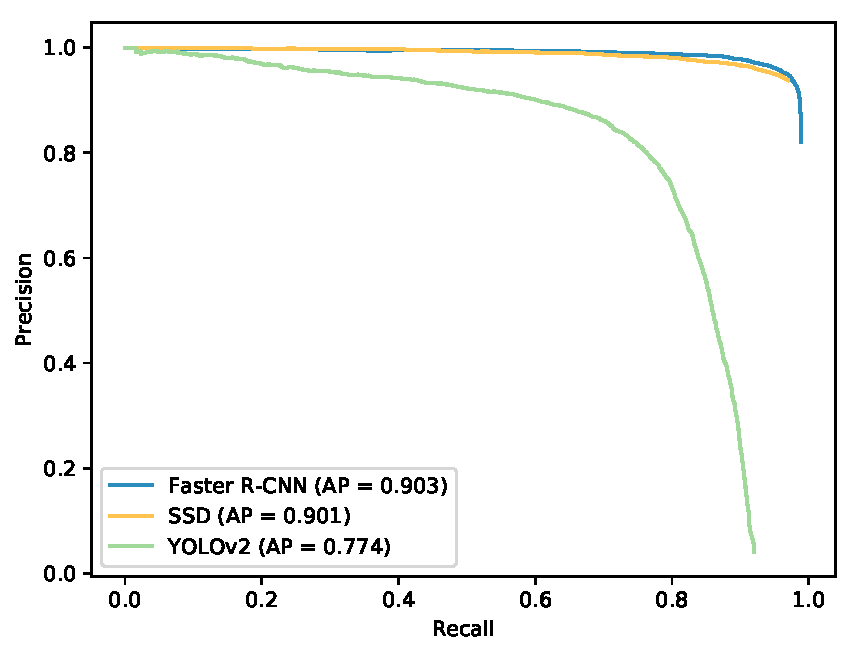
\includegraphics[width=\linewidth]{images/pr_bbox.pdf}
	\caption{Numerical results (AP) of baseline models evaluated with HBB ground truths.}
	\label{fig:pr_bbox}
\end{figure}

\subsection{Baseline with Oriented Bounding Boxes}

Prediction of oriented bounding boxes(OBB) is difficult because the state-of-the-art detection methods are not designed for oriented objects. Therefor, we choose Rotation Region Proposal Networks(RRPN)\cite{RRPN} as the framework for its accuracy and efficiency, then we modify it to adapt UAV-BD on the basis of dataset statistics in section \ref{ssec:Dataset_Statistics}.

For RRPN, it's based on Faster R-CNN, in Faster R-CNN, Region of Interests(RoIs) generated by Region Proposal Network(RPN) are rectangles which can be write as $ R = (x_{min}, y_{min}, x_{max}, y_{max}) = (c_x, c_y, w, h) $. These RoIs have regressed from $ k $ anchors which are generated by some predefined scales and aspect ratios. But in RRPN, it uses predefined scales, aspect ratios and \textit{angles} to generate RoI, so RRPN can predict oriented bounding boxes which can be written as $ R=(c_x, c_y, w, h, \theta) $. In the section \ref{ssec:Dataset_Statistics}, we analyzed the size, aspect ratio and angle distributions of UAV-BD, so we can select reasonable scales, aspect ratios and angles value to generate new anchors which are shown in Fig.\ref{fig:anchors}. 

The experimental results of RRPN prediction are shown in Fig.\ref{fig:result}. In Fig.\ref{fig:result}, forth row illustrates the results for RRPN.



\begin{figure}
	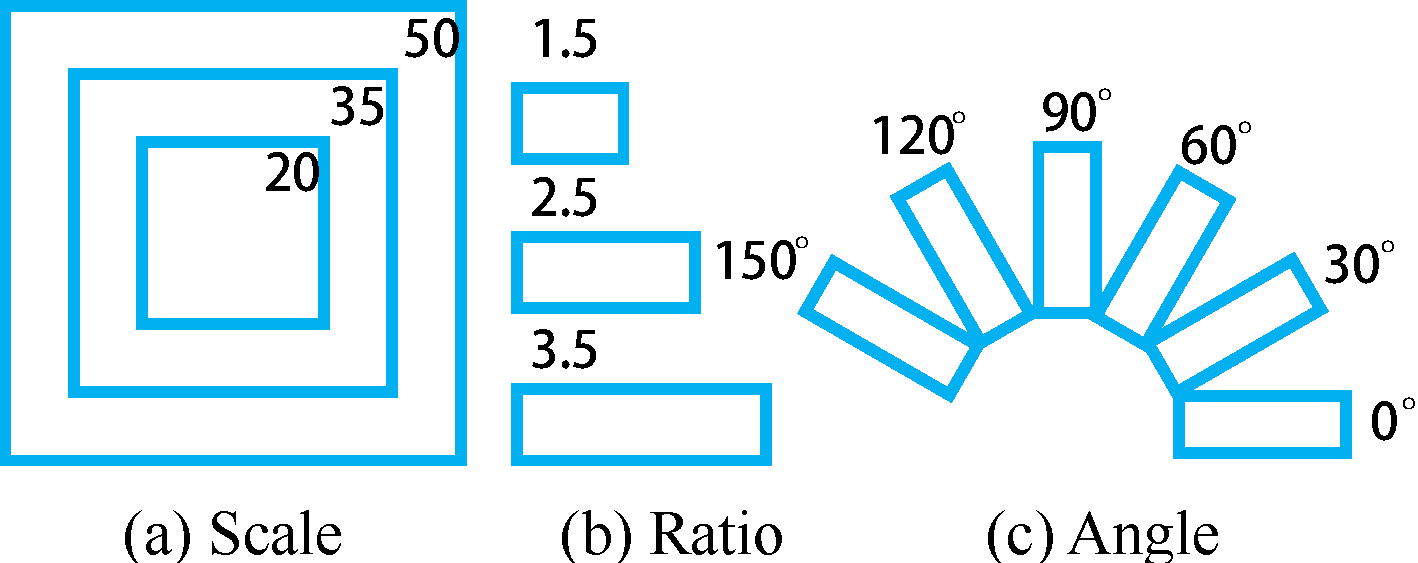
\includegraphics[width=\linewidth]{images/scale_ratio_angle.pdf}
	\caption{Anchor strategy in our framework of RRPN}
	\label{fig:anchors}
\end{figure}

\begin{figure}
	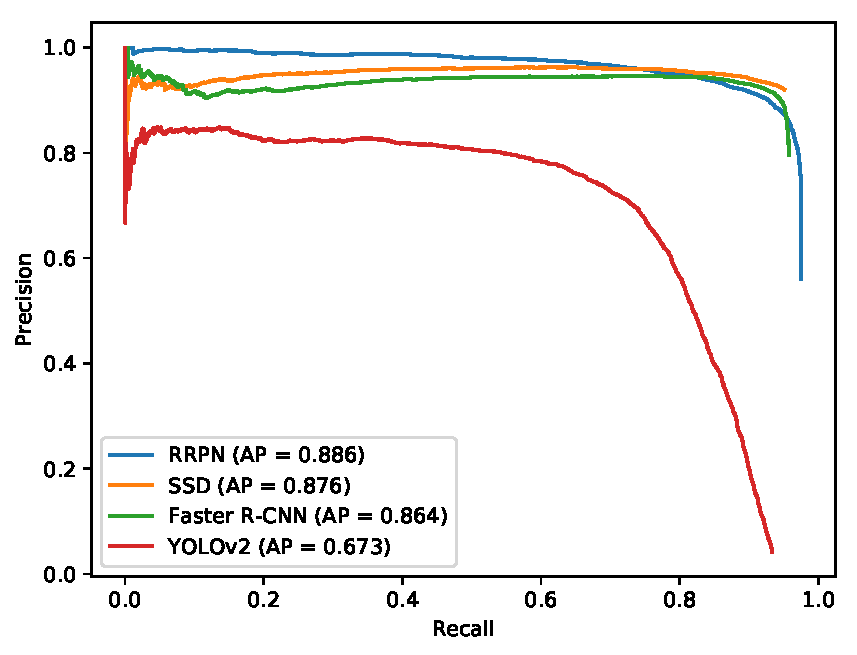
\includegraphics[width=\linewidth]{images/pr_rbbox.pdf}
	\caption{Numerical results (AP) of baseline models evaluated with OBB ground truths.}
	\label{fig:pr_rbbox}
\end{figure}

%\begin{figure}
%	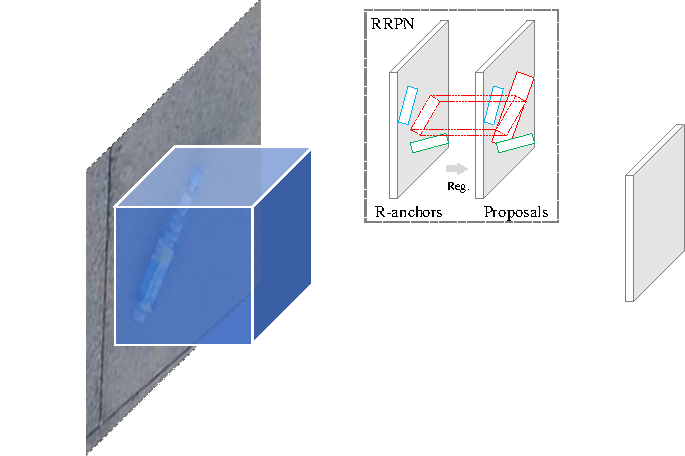
\includegraphics[width=\linewidth]{images/RRPN.pdf}
%	\caption{Rotation based text detection pipline}
%	\label{fig:pipline}
%\end{figure}


\subsection{Experimental Analysis}

Fig.\ref{fig:pr_bbox} show the quantitative comparison result of three baseline models evaluated with HBB ground truth, measured by precision-recall curve and AP values. For evaluation metrics, we adopt the same AP calculation as for PASCAL VOC. As can be seen from it, Faster R-CNN, SSD, YOLOv2 obtain $ 90.3\% $, $ 90.1\% $, $ 77.4\% $ performances, respectively.


Fig.\ref{fig:pr_rbbox} show the quantitative comparison result of five baseline methods evaluated with OBB ground truth, measured by precision-recall curve and AP values. As can be seen from it, RRPN, SSD, Faster R-CNN, YOLOv2, DRBox obtain $ 88.6\% $, $ 87.6\% $, $ 86.4\% $, $ 67.3\% $, $ 32.7\% $ performances, respectively.

In Fig.\ref{fig:result}, we compare the results between objects detection experiments of HBB and OBB. For oriented objects shown in Fig.\ref{fig:result}, location precision of objects in HBB 
experiments are much lower than OBB experiments and results are suppressed through progress operations. So OBB regression is the correct way for oriented object detection that can be really integrated to real applications.


\begin{figure}
	\includegraphics[width=\linewidth]{images/result.png}
	\caption{Visualization results of testing on UAV-BD using well-trained Faster R-CNN, SSD and RRPN. \textbf{TOP} to \textbf{Bottom} respectively illustrate the results for Faster R-CNN, SSD, YOLOv2 and RRPN.}
	\label{fig:result}
\end{figure}










%\begin{figure}
%	\centering
%	\subfigure[angle distribution]
%	{
%		\label{angle}
%		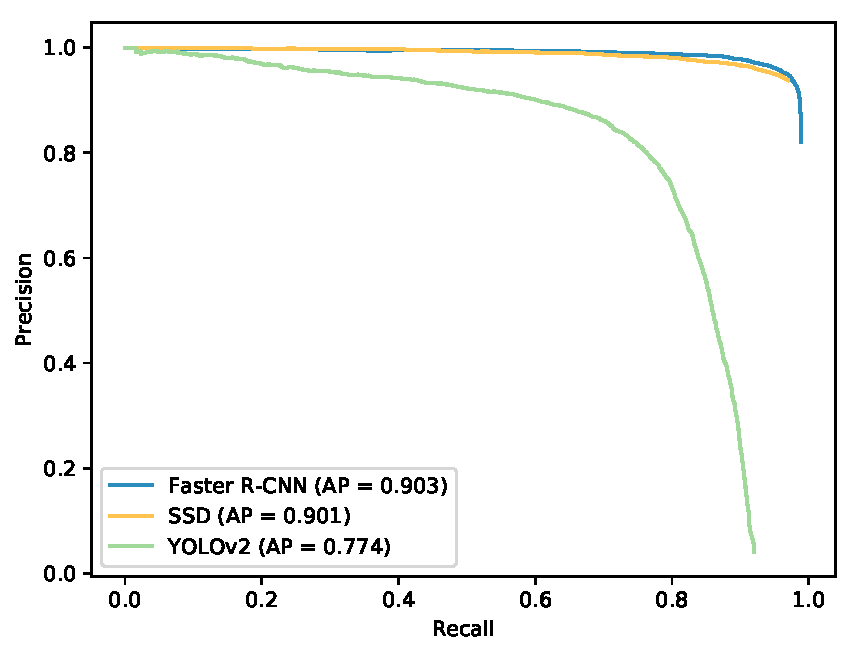
\includegraphics[width=0.45\linewidth]{images/pr_bbox.pdf}
%	}
%	\subfigure[size distribution]
%	{
%		\label{size}
%		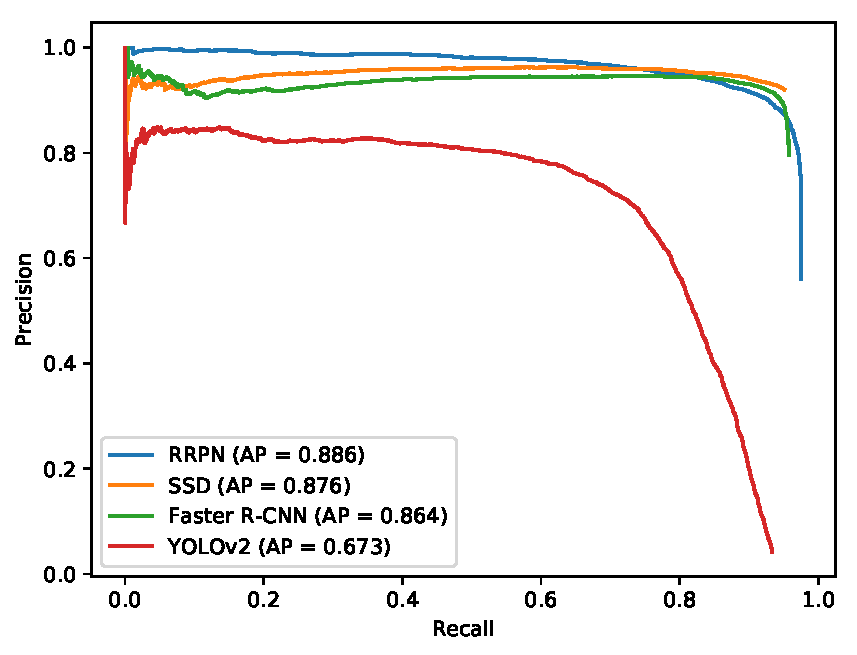
\includegraphics[width=0.45\linewidth]{images/pr_rbbox.pdf}
%	}
%	\caption{The precision-recall curve for bottle detection for Faster R-CNN, SSD and RRPN}
%	\label{fig:PR}
%\end{figure}





%\renewcommand{\algorithmicrequire}{\textbf{Input:}}
%\renewcommand{\algorithmicensure}{\textbf{Output:}}


%\begin{algorithm}
%	\caption{IoU computation}
%	\begin{algorithmic}[1]
%		\Require Rectangle $ R_1, R_2,\cdots,R_N $
%		\State IoU[1, $ N $][1, $ N $] $ \gets $ 0
%		\For {each pair of $ R_i, R_j(i<j) $} 
%		\State Point set $ PSet \gets \emptyset $
%		\State Add intersection points of $ R_i $ and $ R_j $ to $ PSet $
%		\State Add the vertices of $ R_i $ inside $ R_j $ into $ PSet $
%		\State $ \text{IoU}(i,j) \gets (\text{Area}(R_i) + \text{Area}(R_j) - I)/I $
%		\EndFor
%		\Ensure IoU
%	\end{algorithmic}
%\end{algorithm}

